\documentclass{beamer}
\usepackage{animate}
\usepackage{amsmath}
\usepackage{tikz}
\usetheme{Madrid}
\usepackage{tikz}
\usepackage{soul}
\usepackage[normalem]{ulem}
\graphicspath{{./figures/}}

\useinnertheme{circles}
%Information to be included in the title page:
\title{Decision Trees and Random Forrest}
\author{Comp. Bio II}
\date{5th May, 2026}

\renewcommand{\insertshortauthor}{Comp. Bio II}  
\renewcommand{\insertshorttitle}{Decision Trees and Random Forrest}
\renewcommand{\insertshortdate}{5th May, 2026} % Define custom text for 3rd block

\usepackage{amsthm}
\newcommand*{\QED}{\hfill\ensuremath{\blacksquare}}





\begin{document}
	\frame{\titlepage}
	
	
\begin{frame}
		\frametitle{Trees}
		\begin{center}
			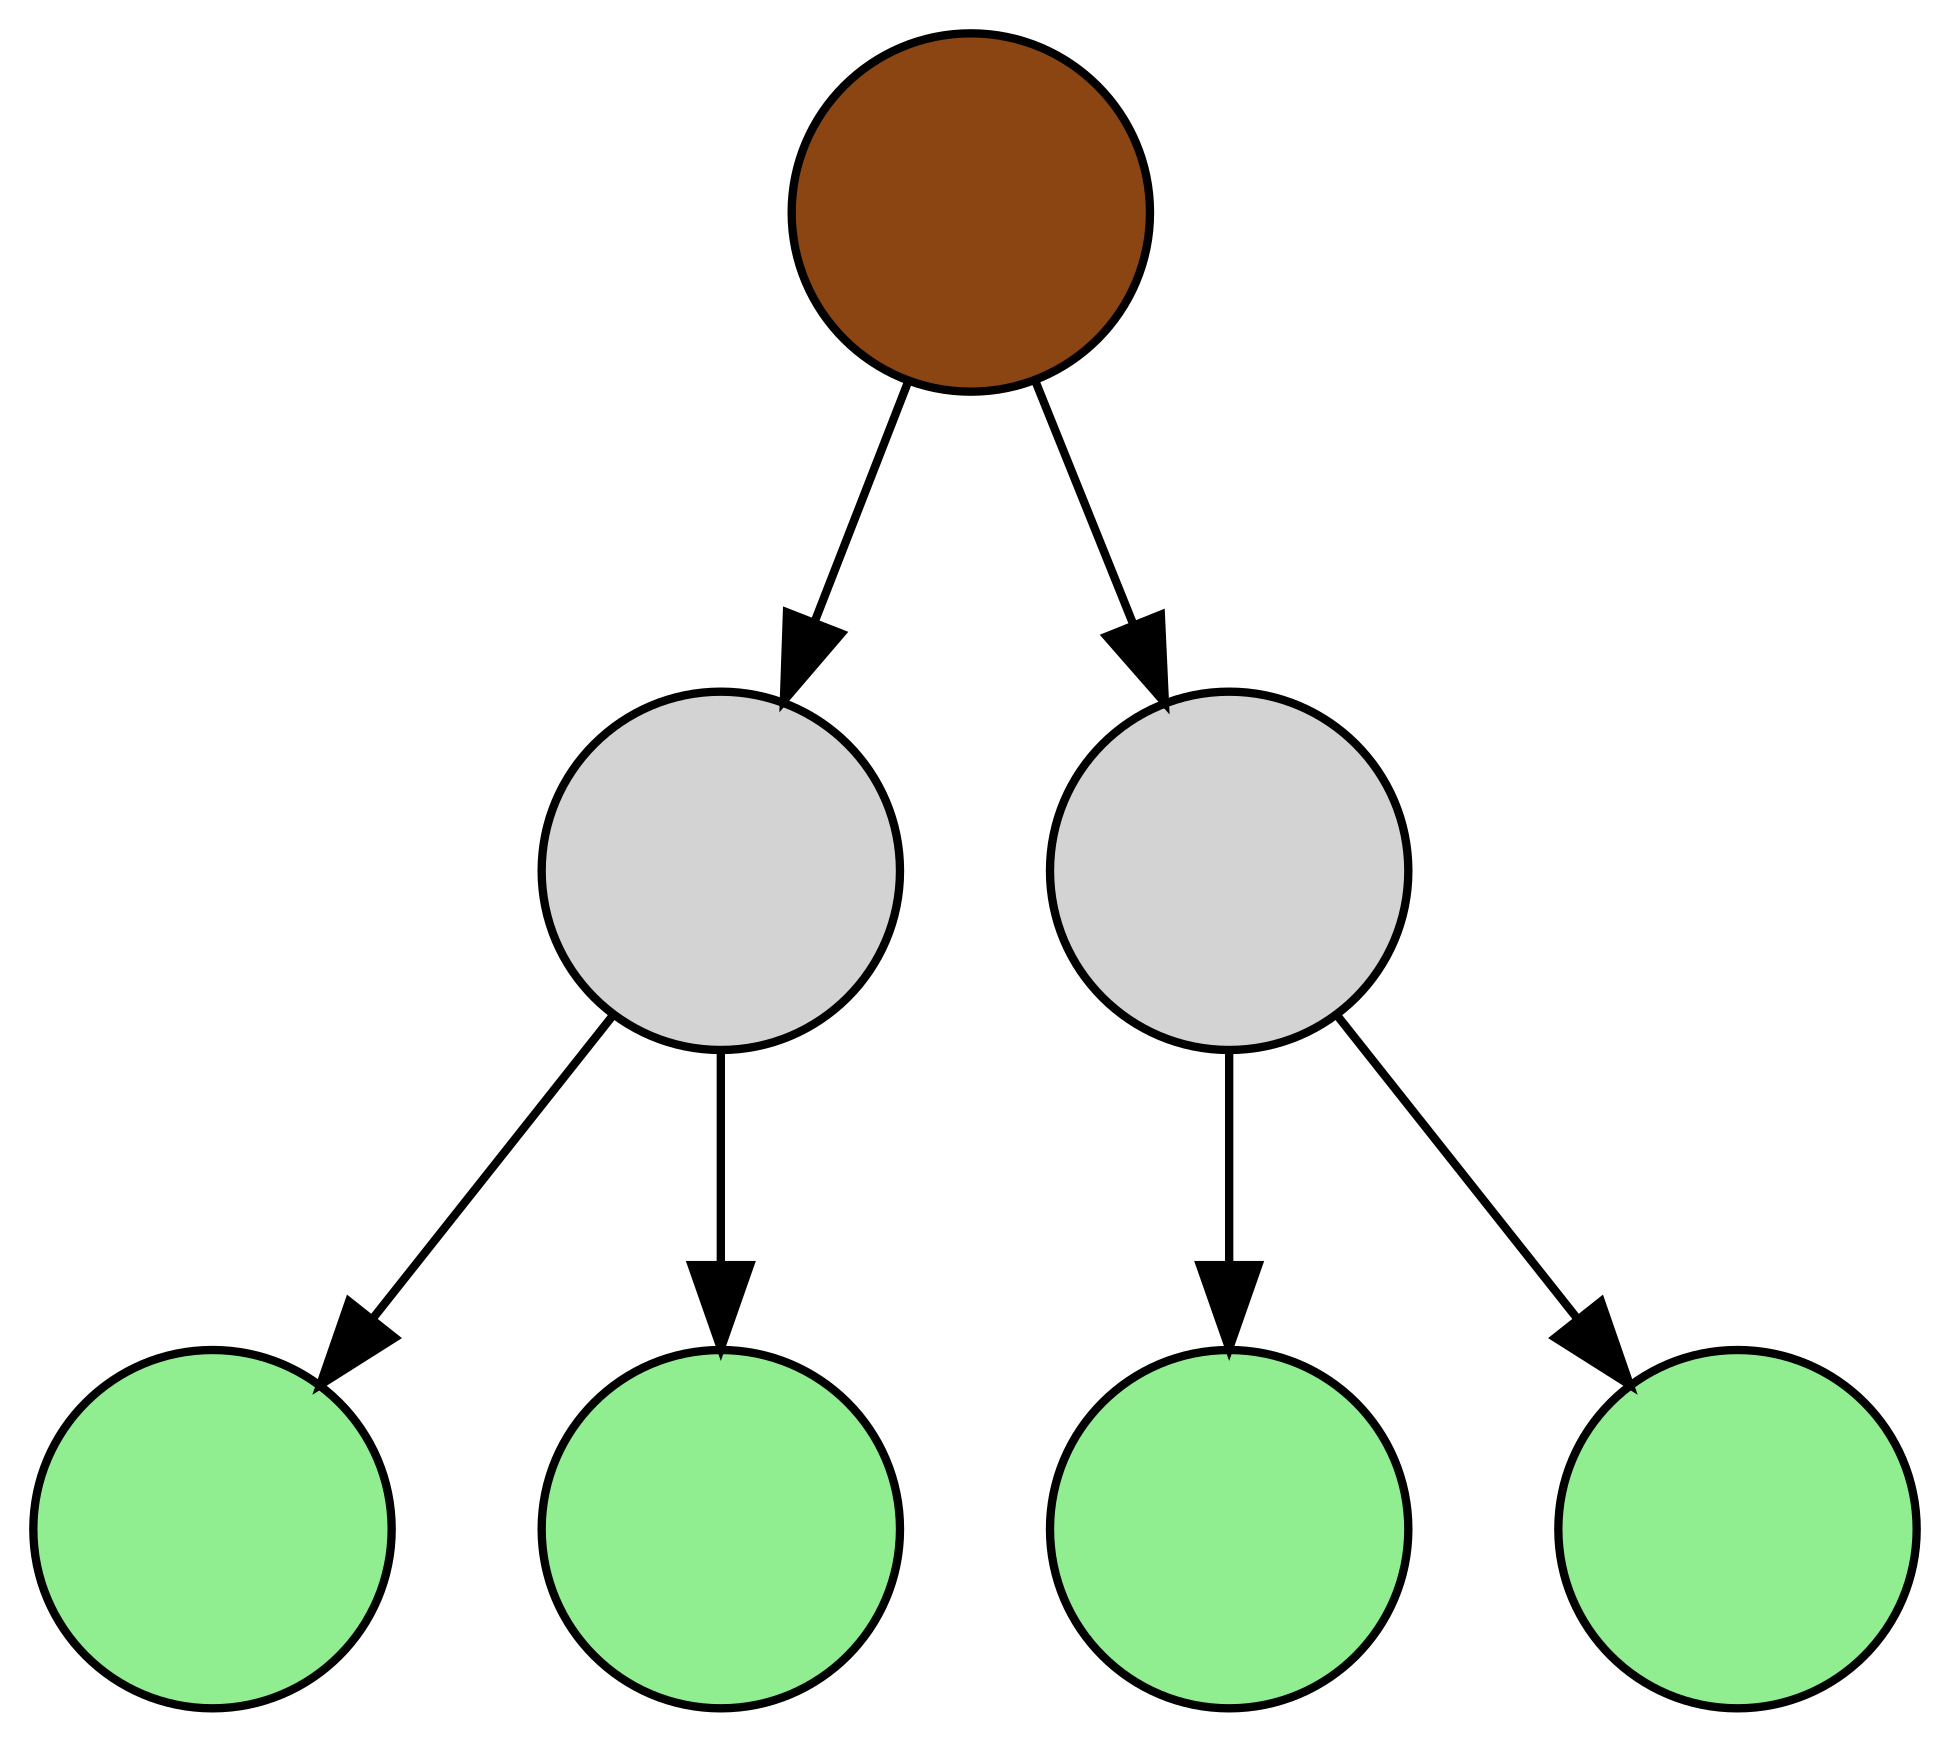
\includegraphics[width=0.35\linewidth]{tree}		
		\end{center}
		
		\begin{itemize}
			\item A \textbf{tree} is a connected graph with no cycles.
			
			\item A \textbf{rooted tree} has a special node called the \textbf{root}.
			
			\item The root has no parent. All other nodes have exactly one parent.			
			
			\item \textbf{Leaves} are nodes with no children.
			
			
		\end{itemize}	
\end{frame}	

\begin{frame}
	\frametitle{Decision tree}
	\centering
	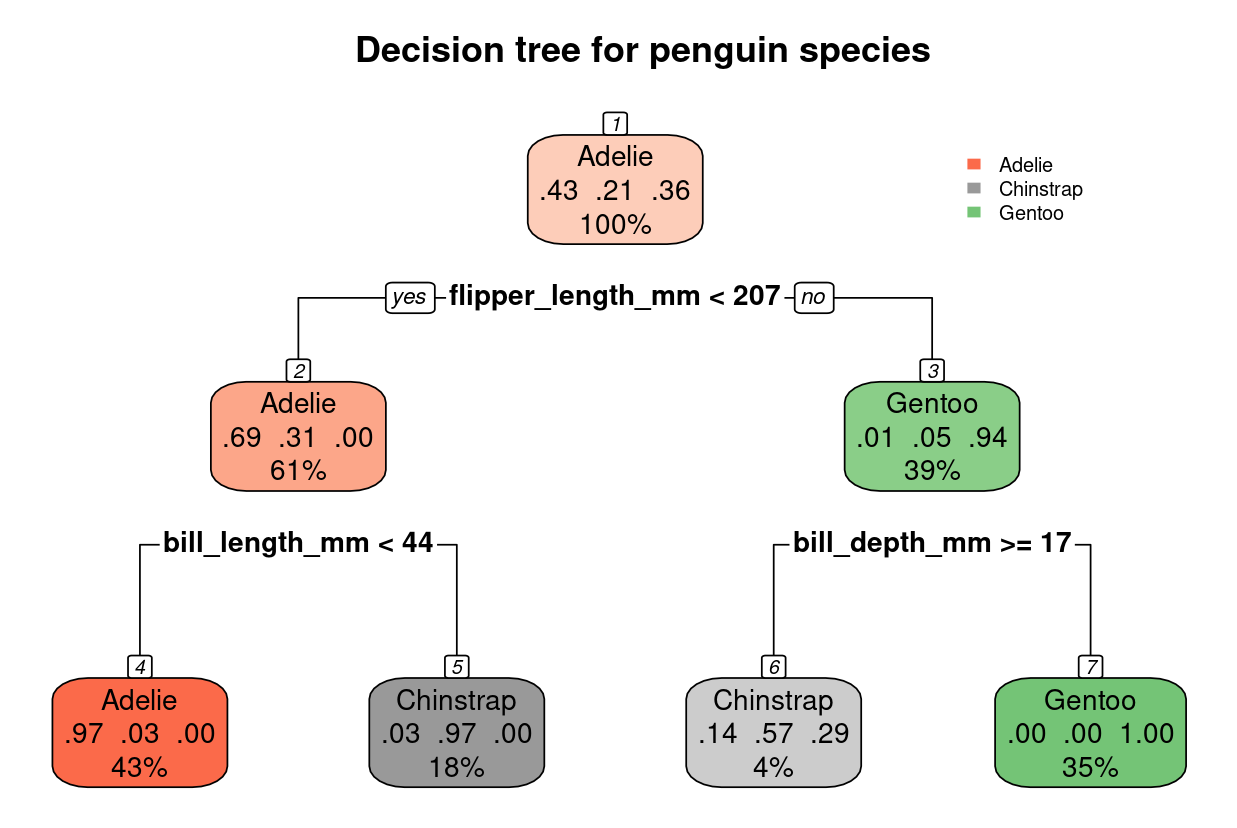
\includegraphics[width=0.6\linewidth]{decision_tree}		
	
	
	\begin{itemize}
		\item Internal nodes split the data based on feature values.
		\item Leaves assign a constant prediction (e.g. class label).
	\end{itemize}
\end{frame}	

\begin{frame}
	\frametitle{Decision tree - visualization}
	\centering
	\includegraphics[width=0.8\linewidth]{ess_tree_visualization.png}
	
	\begin{itemize}
		\item A decision tree models a piecewise constant function.		
		\item Can be used for both regression and classification.
	\end{itemize}
\end{frame}	

	
\begin{frame}
	\frametitle{Training a decision tree}
	
	\begin{itemize}
		\item Start with all data at the root.
		
		\item At each node, consider possible splits of the data.
		\pause
		
		\item Choose the \textbf{best split} according to a criterion:
		\begin{itemize}
			\item Regression: minimize residual sum of squares (RSS)
			\item Classification: minimize impurity (e.g. Gini index)
		\end{itemize}
		\pause
		\item Recursively repeat on resulting subsets.
		
		\item Stop when a stopping criterion is reached (e.g. small nodes).
		
		\pause
		\item Many variations exist (e.g. limiting depth, random feature selection).
	\end{itemize}
	
\end{frame}

\begin{frame}
	\frametitle{Gini index}
	\centering
	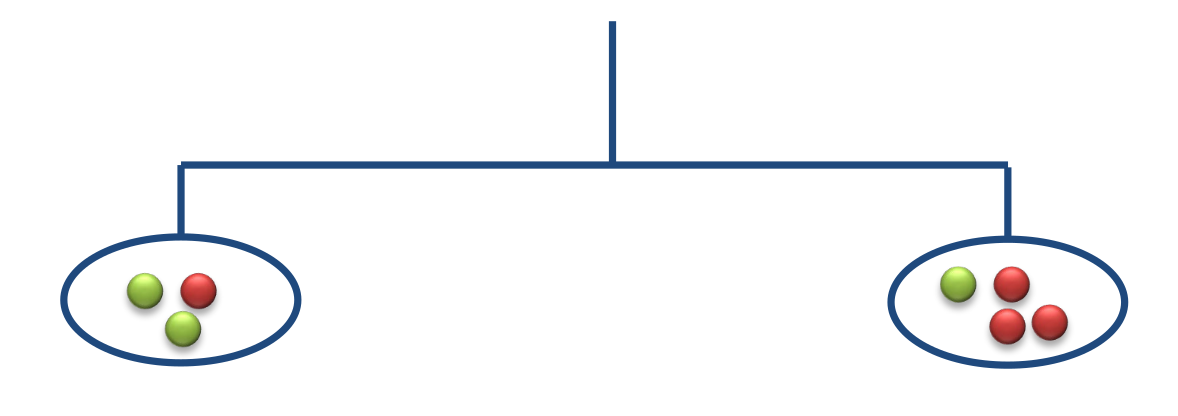
\includegraphics[width=0.6\linewidth]{gini_example}
	
	
	
	\begin{itemize}
		\item Gini index is defined as 
		$$G = 1 - \sum_{k=1}^{K} p_k^2$$
		where $p_k$ is a fraction of k-th class (out of K classes) in the node.	
		
		\item Equals the probability of misclassification (if labels are assigned according to class proportions).
		\item Used to train classification trees.
	\end{itemize}
	
\end{frame}


	
	
	
	
\end{document}
